\chapter{A Game with Assets in SpriteBuilder}

Graphics and Sounds are the essence of every good game. In the first chapter you
have learned the very basics of \SB{} and \cocos{} by building a game that only
uses plain colored shapes. In this chapter you will learn how \SB{} helps you to
integrate assets into your game. Learning by example is the most fun, so we will
build a small game throughout this chapter that uses all aspects of asset
management. 

\section{Adding Assets to a SpriteBuilder project}
Start by creating a new \SB{} project for this game. I have called the
project \textit{FallingObjects}.

Now you should download the assets from
\url{https://dl.dropboxusercontent.com/u/13528538/SpriteBuilderBook/assets.zip}.
Once the download completes you add the assets to the project by dragging the
entire folder into the left \textit{File View} in the left panel of
\SB{}:\index{Assets!Adding Assets}

\begin{figure}[H]
		\centering
		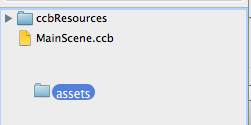
\includegraphics[width=200pt]{images/Chapter2/DragAssets.png}
\end{figure}

Great, now we have some assets to use in our game. Now is a good time to take a
close look at how \SB{} and \cocos{} handle assets.

\section{Asset Handling in \SB{} and \cocos{}}
One of the main goals of \SB{} is to make game development for multiple device
types as easy as possible. This means that games should automatically be able to
run on differently sized iPhones, iPads and Android Devices. Since each of these
devices has a different resolution \cocos{} and \SB{} allow developers to use different assets to target them. \SB{}
provides four different resolution categories:
\begin{description}
\item[phone] resolution for non-retina iPhone and Android devices
\item[phone-hd] retina resolution for iPhone and Android
\item[tablet] resolution for non-retina iPad and Android tablets
\item[tablet-hd] resolution for retina iPad and Android tablets
\end{description}

Luckily using \SB{}, there is no need to provide four resolutions for each asset
thanks to \textbf{automatic downscaling}\index{Assets!Automatic Downscaling}.
Per default \SB{} assumes that all assets added to a project are provided in \textit{tablet-hd} resolution, then
\SB{} generates downscaled images for the other resolutions. While you can
provide different images for four targets, \SB{} only knows three resolution
types:
\begin{description}
\item[1x] non-retina images
\item[2x] retina images
\item[4x] tablet retina images
\end{description}

By default \SB{} maps these resolution types to the different devices in a way
that every asset has the same size (in relation to the screen size) on every
device. This means games running on an iPad will look very similar to games
running on an iPhone, except that the have a slightly different aspect ratio.
Here is an example from on of our tutorials showing what a game looks like on
different device types:

\begin{figure}[H]
		\centering
		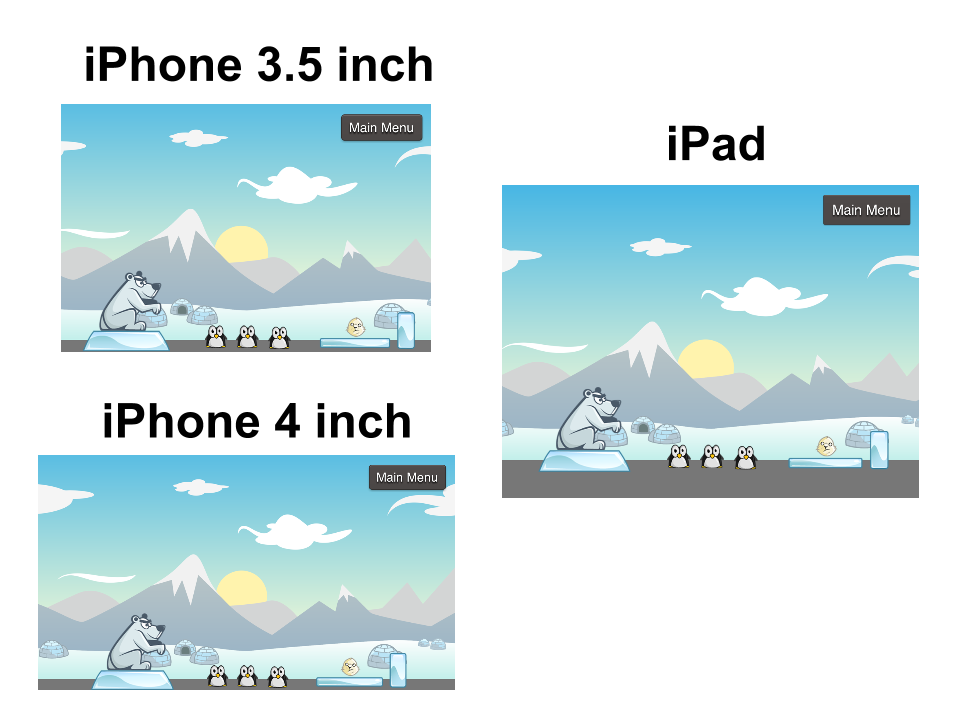
\includegraphics[width=0.9\linewidth]{images/Chapter2/ResultsFlexibleScaleMode.png}
		\caption{From our tutorial \textit{Dynamic Layouts with SpriteBuilder and
		Cocos2D}}
\end{figure}

Let's take a look at where all the settings I mentioned are visible in the \SB{}
UI. When you open the project settings (\textit{File -> Project Settings\ldots})
you can see the available downscaling options:

\begin{figure}[H]
		\centering
		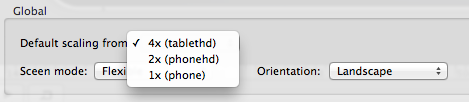
\includegraphics[width=300pt]{images/Chapter2/DownScalingGlobal.png}
\end{figure}

This setting defines the \textit{global} downscaling option. Individual assets
can define their own behaviour, thereby overriding this global setting. To make
support of multiple devices as easy as possible you should provide all of your
assets in \textit{4x} resolution and keep this default setting.

When you select an individual asset from the File View you can see different
downscaling settings:

\begin{figure}[H]
		\centering
		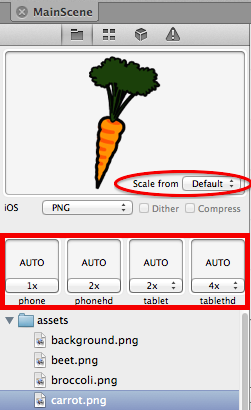
\includegraphics[height=200pt]{images/Chapter2/DownScalingPerAsset.png}
\end{figure}

Each asset can have its own \textit{Scale from} setting. \textit{Default} means
that the global project setting applies (in this project: downscaling from
\textit{4x}). Additionally you can see how the different resolution types are
mapped to the different device types. Here you could for example choose that a
certain asset should not be scaled up on retina tablets by choosing a
\textit{2x} resolution for \textit{tablethd} - however, the default settings
work best most of the time.

For future reference, this is an example that shows you which sizes your assets
will have on the different devices by default:

\begin{table}[H]
\begin{tabular}{llll}
\textbf{Device} & \textbf{Default Resolution Type} & \textbf{Size on Screen (points)} & \textbf{Size in Pixels} \\
iPhone          & 1x                               & 50x50                            & 50x50                   \\
iPhone Retina   & 2x                               & 50x50                            & 100x100                 \\
iPad            & 2x                               & 100x100                          & 100x100                 \\
iPad Retina     & 4x                               & 100x100                          & 200x200                
\end{tabular}
\end{table}

You can see, if you have a size in mind for a certain asset on an iPhone you
should provide the asset in four times larger resolution.

A last interesting case are background images that you want to work for
all 4 resolutions. A solution is discussed in
the Q\&A section (\ref{background_all_resolutions}).

\begin{details}[frametitle={Different images for different devices}] 
You can not only change the scaling option for an asset on different devices,
you can even use an entirely different image for a certain resolution. You can
do that by dragging an image \textbf{that is currently not part of the \SB{}
project} from Finder into one of the four boxes below the asset preview:
%TODO: note this fact in docs as well
%TODO: ask viktor why this displays the image for tablet and not for phone in SB
\begin{figure}[H]
		\centering
		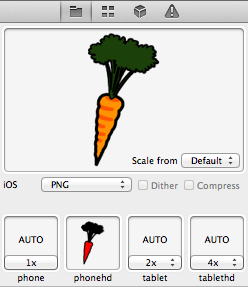
\includegraphics[height=200pt]{images/Chapter2/DifferentImageDevice.png}
\end{figure}

Note that images you add this way will be displayed in exactly the size you have
added them and will not be downscaled.

\end{details}

\begin{details}[frametitle={Behind the scenes}] 
If you are interested in how \SB{} and \cocos{} organize assets you can take a
look at the resource package
(\textit{/Packages/\allowbreak{}SpriteBuilder Resources\allowbreak{}.sbpack}) by
right-clicking and selecting \textit{Show Package Contents}:
\begin{figure}[H]
		\centering
		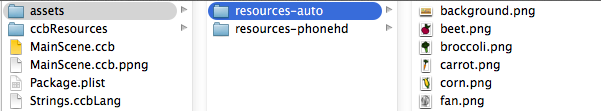
\includegraphics[width=280pt]{images/Chapter2/behindscenes_resourcepack.png}
\end{figure}
You will see that \SB{} groups images inside the assets folder into a
\textit{resources-auto} folder, all images in that folder are subject to
automatic downscaling. If you explicitly add images for a certain resolution as
shown with the carrot in the above example, a new folder for that resolution
(e.g. \textit{resources-phonehd}) is created.

In \cocos{} a class called \inlinecode{CCFileUtils} is responsible for loading
the correct images for the current device during runtime. \SB{} uses a special
configuration of \inlinecode{CCFileUtils} that is set up in
\inlinecode{[CCBReader configureCCFileUtils]}. \index{Framework
Classes!CCFileUtils}
\end{details}

\section{Adding the background image}
Now that we have a basic understanding of how asset management works, lets get
started working on our game. For now our game will only consist of one scene, so
we can start working in the \textit{MainScene.ccb} that is part of the \SB{}
template. First, remove the existing content so that we can start with a blank
scene. Now we can add the background image. To add a sprite to a scene we can
simply drag the asset to the stage, \SB{} will automatically create an instance
of \ccsprite{}. Add the \textit{background.png} image to the stage.

%mention document types
%mention position type
